\documentclass[a4j,10.5pt]{jreport}
\usepackage[dvipdfmx]{graphicx}
\usepackage{amssymb}
\usepackage{amsmath}
\usepackage{float}
\usepackage{here}


% \usepackage{tabularx}
% \usepackage{multirow}
% \usepackage{slashbox} default commented out
\usepackage{cite}
% \usepackage{supertabular}
% \usepackage{jtygm} default commented out

\makeatletter %% プリアンブルで定義する場合は必須

% \setcounter{secnumdepth}{5}

%\newcommand{\figcaption}[1]{\def\@captype{figure}\caption{#1}}
%\newcommand{\tblcaption}[1]{\def\@captype{table}\caption{#1}}



%---------------------------------------------------------------------
%\setcounter{topnumber}{5}%    ページ上部の図表は 5 個まで
%\def\topfraction{1.00}%       ページの上 1.00 まで図表で占めて可
%\setcounter{bottomnumber}{5}% ページ下部の図表は 5 個まで
%\def\bottomfraction{1.00}%    ページの下 1.00 まで図表で占めて可
%\setcounter{totalnumber}{10}% ページあたりの図表は 10 個まで
\def\textfraction{0.2}%        ページのうち本文が占める割合の下限
%        これを 0 にすると本文が 1 行だけのページが出来る
%        0.04 くらいにするとS 1 行だけのページは防げる
%        0.1 くらいが良いかも知れない
\def\floatpagefraction{0.8}%   図表だけのページは少ないかも
                           %   これだけを図表が占める
%---------------------------------------------------------------------

\renewcommand{\bibname}{参考文献}


\makeatother %% プリアンブルで定義する場合は必須

\begin{document}

\begin{titlepage}

\vspace{40mm}
\begin{center}
{\Large 平成31年度\\卒業論文}\\[80mm]
\end{center}

\begin{center}
{\huge 歩行時における足の接地推定}\\[80mm]
\end{center}

\begin{flushright}
{\large s163043 鈴木健太}\\[1mm]
{\large 平成28年度入学}\\[1mm]
{\large 島根大学 総合理工学部 数理・情報システム学科}\\[1mm]
{\large 情報システムコース}\\[8mm]
{\large 主指導教員: 平川 正人 教授}\\[3mm]
{\large 提出日:令和2年1月24日}\\%
\end{flushright}
\end{titlepage}

\newpage
% \pagenumbering{roman}

\chapter*{概要}
人の動作の計測,解析は運動力学やヒューマンコンピュータインターフェースなど様々な分野に応用されている.特に,人の動作の中でも歩容解析は,最も注目されている研究テーマの一つである.体組成の推定\cite{cite1},個人識別,トレーニングやリハビリテーション,転倒予防などに歩容解析が役立てることができる.歩容解析を行う上で,対象に関するあるパラメータを測定する.このパラメータは大きく分けて次の2つである.1つは空間的パラメータである.これはステップ長,スライド長などが含まれる.1つは時間的パラメータである.これは立脚期,遊脚期\cite{cite2}など歩行の1周期の中の足の位置に着目し各時間帯を分類したパラメータである.

本研究では,姿勢推定ライブラリの1つであるPoseNetを用いて,
歩行時における各特徴点の値を解析し非侵襲で両脚支持相を抽出することを目指す.実験では,フーリエ解析を用い,姿勢推定から得られた情報で両脚支持相を抽出できる可能性を示した.
\addcontentsline{toc}{chapter}{概要}

\section*{Abstract}
Measurement and analysis of human movements are applied to various fields such as kinematics and human-computer interface. In the field of human motion analysis, Analysis of walking motion: Gait analysis is one of the most attractive research topics. Gait analysis can be useful for estimation of human body composition, personal identification, training and rehabilitation, fall prevention, etc. When performing gait analysis, certain parameters related to the object are measured. This parameter is roughly divided into the following two. One is a spatial parameter. This includes step length, slide length, etc. One is a temporal parameter. This is a parameter that classifies each time zone by focusing on the position of the foot in one cycle of walking such as stance phase and swing phase.

In this study, we use PoseNet, one of the pose estimation libraries, to analyze the value of each keypoints during walking and extract the double legs supporting phase in a non-invasive manner. In experiments, it was shown that Fourier analysis could be used to extract the double legs supporting phase from information obtained from posture estimation.
\pagenumbering{roman}

\tableofcontents

\listoftables %表目次

\listoffigures %図目次

\baselineskip = 8mm

\clearpage

\pagenumbering{arabic}


% 必要に応じてchapter,sectionを追加・変更する.

\chapter{はじめに}
\section{研究背景}
人の動作の計測,解析は運動力学やヒューマンコンピュータインターフェースなど様々な分野に応用されている.特に,人の動作の中でも歩容解析は,最も注目されている研究テーマの一つである.体組成の推定,個人識別,トレーニングやリハビリテーション,転倒予防などに歩容解析が役立てることができる.歩容解析を行う上で,対象に関するあるパラメータを測定する.このパラメータは大きく分けて次の2つである.1つは空間的パラメータである.これはステップ長,スライド長などが含まれる.1つは時間的パラメータである.これは立脚期,遊脚期\cite{cite1}など歩行の1周期の中の足の位置に着目し各時間帯を分類したパラメータである.

本研究では,姿勢推定ライブラリの1つであるPoseNetを用いて,
歩行時における各特徴点の値を解析し非侵襲で両脚支持相を抽出することを目指す.
\section{研究目的}

\section{本論文の構成}

\chapter{関連研究}
\section{歩行位相分割に関する研究}
\section{歩容解析の応用に関する研究}

参考\cite{cite1}.

\chapter{提案手法}
\section{データ収集}
対象が1人であり,自然な歩行を足全体が写るように横方向から撮影した.
この映像に対し,PoseNetを用い姿勢推定を行い手首,膝,足首の左右計6箇所の特徴点からデータを収集した.サンプリングは約$28\,\mathrm{hz}$で,特徴点の画素の位置よりそれぞれ左右の手首,膝,足首について行われた.PoseNetは機械学習用ライブラリのtensorflow.jsの一部なのでjavascript上で動作する.よって今回の研究では,図\ref{fig:datecollect}のようにlocal環境でjavascriptプログラムを実行し歩行時の映像から特徴点の座標を推定し,csv形式で保存した.収集されたデータはそれぞれパラメータとして時間,x座標,y座標の3つを持つ.
\begin{figure}[H]
  \centering
  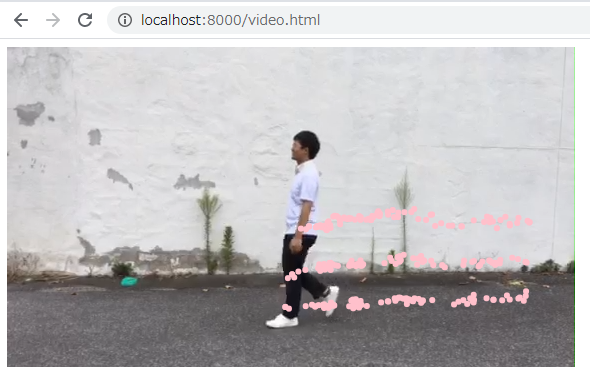
\includegraphics[width=10cm]{figs/datacollect1.png}
  \caption{データ収集画面}\label{fig:datecollect}
\end{figure}


\section{データ分析}
生データ:図\ref{fig:originaldata}のままでは周期性が見出せない.【観察による歩行分析】より歩行周期において立脚期の初期状態イニシャルコンタクト,床への足接地の瞬間と遊脚期の最後であるターミナルスタンス,床に足が着く直前の2つの相は足関節がニュートラル・ゼロ・ポジションである.ニュートラル・ゼロ・ポジションは,足がまっすぐに伸びた状態であり,左右の膝の間の距離は最大になる.であるから,取得したデータにおいても距離を求めることによって周期性が見られると考え,手首,膝,足首のそれぞれに対し左右間のユークリッド距離$L$ を求めた.$L$から図\ref{fig:lengthdata}が得られる.
% \begin{equation}
%   L = \{(x_{left} - x_{right})^2 + (y_{left} - y_{right})^2\}
% \end{equation}
\begin{figure}
    \centering
    \includegraphics{}
    \caption{生データ}
    \label{fig:originaldata}
\end{figure}
\begin{figure}
    \centering
    \includegraphics{}
    \caption{左右関節間距離}
    \label{fig:lengthdata}
\end{figure}
\begin{enumerate}
    \item サンプル
    \item サンプル
\end{enumerate}

\subsection{subsection}

\chapter{システム評価、実験}

\chapter{実験結果、評価、分析等}

\chapter{終わりに、まとめ等}

\chapter*{謝辞}
\addcontentsline{toc}{chapter}{謝辞}
ここに研究の謝辞.主にご協力いただいた方など.


% \bibliographystyle{jplain}
\begin{thebibliography}{99}
  \bibitem{cite1} 畠中泰彦 歩行分析・動作分析のグローバル・スタンダード─最近の知見と治療に役立つ分析のポイント─ 理学療法学 第 40 巻第 8 号 567 ~ 572頁(2013年)
  \bibitem{cite2} 廖若辰,守脇幸佑,槇原靖,村松大吾,武村紀子,八木康史 歩行映像解析による体組成推定に関するー検討 研究報告コンピュータビジョンとイメージメディア(CVIM) Vol.2019-CVIM-218 NO.17

 % \bibitem{cite3} 江原義弘 歩行分析の基礎—正常歩行と異常歩行— 日本義肢装具学会誌 2012 年 28 巻 1 号 p. 57-61
\end{thebibliography}
\addcontentsline{toc}{chapter}{\bibname}

\chapter*{付録}
\addcontentsline{toc}{chapter}{付録}

\end{document}
